\documentclass[../main.tex]{subfiles}

\begin{document}
    \section{Tujuan}
        \begin{enumerate}
            \item Memahami mengenai teori LQR
            \item Memahami pengaruh variabel kendali Q dan R terhadap performansi sistem
            \item Memahami serta mampu merancang kendali LQR
        \end{enumerate}
    \section{Dasar Teori}
        Sistem kendali yang baik merupakan sistem kendali yang memiliki respon transien yang cepat, stabil, dan tidak memerlukan energi yang berlebih. pada perancangan kendali \textit{pole placement}, seluruh proses perancangan difokuskan pada performansi sistem tanpa melihat usaha yang dibutuhkan untuk mencapai nilai tujuan. Pada praktikum ini, dilakukan perancangan kendali optimal yang didasari optimasi terhadap indeks performansi yang telah ditentukan. Indeks performansi dipilih berdasarkan \textit{state} yang akan dioptimalkan. Indeks performansi kuadratis dapat dihitung dengan persamaan berikut.
        \begin{equation}
            J = \int_{0}^{\infty}(x^TQx+u^TRu)dt
            \label{persamaan_1}
        \end{equation}
        \begin{center}
            Keterangan :
            \begin{minipage}[c]{13cm}
                \item $x^T$ : \textit{Conjugate} transpose dari matriks state x
                \item $Q$ : Matriks simterik real definit positif (atau semi definit positif)
                \item $R$ : Matriks real definit positif
                \item $u$ : vektor kontrol
            \end{minipage}
        \end{center}
        Nilai elemen matriks Q dan elemen matriks R diatur untuk menghasilkan sinyal kendali $u = -kx$ yang optimal untuk setiap kondisi awal $x(0)$. Dari hasil persamaan \textit{state space} sistem dan indeks performansi $J$. didapat nilai matriks K yang optimal untuk indeks performansi yang dipilih. nilai $K$ dapat dihitung dengan persamaan berikut,
        \begin{equation}
            K = R^{-1}B^TP
            \label{persamaan_2}
        \end{equation}
        Matriks $P$ merupakan solusi persamaan matriks Ricatti yang tereduksi dan dapat direpresentasikan dengan persamaan berikut,
        \begin{equation}
            A^T P+PA-PBR^{-1} B^T P+Q=0
            \label{persamaan_3}
        \end{equation}
    \section{Hasil dan Pembahasan}
        \subsection{Latihan Satu}
            Dilakukan analisis pada pemodelan \textit{state space} sebagai berikut,
            \begin{equation}
                \begin{bmatrix} \dot{x_1} \\ \dot{x_2} \end{bmatrix} = \begin{bmatrix} -1 & 1 \\ 0 & 2\end{bmatrix} \begin{bmatrix} x_1 \\ x_2 \end{bmatrix} + \begin{bmatrix} 1 \\ 0\end{bmatrix} u
                \label{persamaan_4}
            \end{equation}
            \subsubsection{Analisis Nilai P dan K pada Sistem}
                Nilai P didapatkan dari persamaan berikut,
                \begin{equation}
                    A^T P+PA-PBR^{-1} B^T P+Q = 0 \\[5pt]
                    \label{persamaan_5}
                \end{equation}
                Pemodelan \textit{state space} pada Persamaan \eqref{persamaan_4} dianalisis dengan rumus pada Persamaan \eqref{persamaan_5} sebagai berikut,
                \begin{equation}
                    \begin{split}
                        \begin{bmatrix} -1 & 1 \\ 0 & 2 \end{bmatrix}^T \begin{bmatrix} P_{11} & P_{12} \\ P_{12} & p_{22} \end{bmatrix} + \begin{bmatrix} P_{11} & P_{12} \\ P_{21} & P_{22} \end{bmatrix} \begin{bmatrix} -1 & 1 \\ 0 & 2 \end{bmatrix} - &\\ \begin{bmatrix} P_{11} & P_{12} \\ P_{12} & P_{22} \end{bmatrix} - \begin{bmatrix} P_{11} & P_{12} \\ P_{12} & P_{22} \end{bmatrix}\begin{bmatrix} 1 \\ 0 \end{bmatrix} \begin{bmatrix} 1 \end{bmatrix}^{-1}\begin{bmatrix} 1 \\ 0 \end{bmatrix}^T \begin{bmatrix} P_{11} & P_{12} \\ P_{12} & P_{22} \end{bmatrix} +  \begin{bmatrix} 1 & 0 \\ 0 & 1 \end{bmatrix} &= \begin{bmatrix} 0 & 0 \\ 0 & 0 \end{bmatrix}\\[10pt]
                        \begin{bmatrix} -P_{11}^2 - 2P_{11} + 1 & P_{11} + P_{12} - P_{11} P_{12} \\ P_{11} + P_{12} - P_{11} P_{12} & -P_{12}^2 + 2 P_{12} + 4P_{22} + 1 \end{bmatrix} &= \begin{bmatrix} 0 & 0 \\ 0 & 0 \end{bmatrix}
                        \label{persamaan_6}
                    \end{split}
                \end{equation}
                Dari persamaan \eqref{persamaan_6} dapat dianalisis untuk mencapatkan nilai $P$ sebagai berikut,
                \begin{equation}
                    \begin{split}
                        -P_{11}^2-2P_{11}+1 &= \frac{-(2) \pm \sqrt{(-2)^2 + 4(-1)(1)}}{2(-1)}\\[5pt]
                        P_{11} &= \frac{2 \pm 2.828}{-2} \rightarrow P_{11} = -2.414 \text{ atau } 0.414 \\[10pt]
                        P_{11} + P_{12} - P_{11} P_{12} &= 0 \\[5pt]
                        0.414 + P_{12} - 0.414 P_{12} &=0 \\[5pt]
                        P_{12} &= - 0.706 \\[10pt]
                        -P_{12}^2 + 2P_{12} + 4P_{22} + 1 &= 0 \\[5pt]
                        0.706^2 + 2(-0.706) + 4P_{22} + 1 &= 0 \\[5pt]
                        P_{22} &= -0.021
                        \label{persamaan_7}
                    \end{split}
                \end{equation}
                Nilai - nilai $P$ yang ada pada persamaan \eqref{persamaan_7} dapat disatukan dalam satu matriks sebagai berikut,
                \begin{equation}
                    \begin{split}
                        P = \begin{bmatrix} 0.414 & -0.706 \\ -0.706 & -0.021 \end{bmatrix}
                        \label{persamaan_8}
                    \end{split}
                \end{equation}
                Dari matriks $P$ pada Persamaan \eqref{persamaan_8} dapat dilakukan analisis untuk mencapatkan nilai $K$ sebagaimana ditunjukkan pada Persamaan \eqref{persamaan_9}
                \begin{equation}
                    \begin{split}
                        K &= R^{-1} B^T P \\[5pt]
                        K &= 1^{-1} \begin{bmatrix} 1 \\ 0 \end{bmatrix}^T \begin{bmatrix} 0.414 & -0.706 \\ -0.706 & -0.021\end{bmatrix} \\[5pt]
                        K &= \begin{bmatrix} 0.414 & -0.706 \end{bmatrix} \\[5pt]
                        \label{persamaan_9}
                    \end{split}
                \end{equation}
            \subsubsection{Verifikasi Analisis Menggunakan Matlab}
                Sistem dapat dikendalikan dengan metode \textit{full state feedback} apabila sistem dalam keadaan \textit{controllable}. Untuk menguji apakah sistem dalam keadaan \textit{controllable} atau tidak dilakukan pengujian terhadap sistem dengan kode program berikut,
                \lstinputlisting[language=matlab]{assets/code/LQR_CRTB.m}
                Hasil dari kode program diatas sebagai berikut,
                \lstinputlisting[language=matlab]{assets/code/CONSOLE_CRTB.m}
                Dari hasil kode tersebut, dapat dilihat bahwa sistem merupakan sistem yang bersifat \textit{uncontrollable} karena rank matriks dari sistem tidak sama dengan \textit{state} pada sistem.
        \subsection{Latihan Dua}
            Dilakukan analisis kendali LQR pada pemodelan \textit{state space} sebagai berikut,
            \begin{equation}
                \begin{split}
                    \begin{bmatrix}\dot{x_1} \\ \dot{x_2} \end{bmatrix} &= \begin{bmatrix} 0 & 1 \\ 0 & -1 \end{bmatrix} \begin{bmatrix} x_1 \\ x_2 \end{bmatrix} + \begin{bmatrix}0 \\ 1\end{bmatrix}u \\[5pt]
                y &= \begin{bmatrix} 1 & 0 \end{bmatrix} \begin{bmatrix} x_1 \\ x_2 \end{bmatrix}
                \label{persamaan_10}
                \end{split}
            \end{equation}
            \subsubsection{Controllability Test}
                Untuk mengetahui apakah sistem dapat dikendalikan atau tidak dapat menggunakan \textit{controllability test} sebagai berikut,
                \textit{Controllability}
                \begin{equation}
                    \begin{split}
                        C_m &= \begin{bmatrix} A & AB \end{bmatrix} \\[5pt]
                        C_m &= \begin{bmatrix} 0 \\ 1 \end{bmatrix} \begin{bmatrix} 0 & 1 \\ 0 & -1\end{bmatrix} \begin{bmatrix}0 \\ 1 \end{bmatrix} \\[5pt]
                        C_m &= \begin{bmatrix} 0 & 1 \\ 1 & -1
                        \end{bmatrix}
                        \label{persamaan_11}
                    \end{split}
                \end{equation}
                Hasil dari analisis terhadap sistem menunjukkan sistem masih dapat dikendalikan karena memiliki rank matriks tidak sama dengan nol.
            \subsubsection{Perancangan Kendali Full State Feedback}
            Perancangan kendali dilakukan dengan melakukan analisis pada sistem untuk mendapatkan  nilai P. analisis menggunakan persamaan berikut,
            \begin{equation}
                A^T P+PA-PBR^{-1} B^T P+Q = 0
                \label{persamaan_12}
            \end{equation}
            Pemodelan \textit{state space} sistem pada Persamaan \eqref{persamaan_10} dianalisis menggunakan Persamaan \eqref{persamaan_12} sebagai berikut,
            \begin{equation}
                \begin{split}
                    \begin{bmatrix} 0 & 1 \\ 0 & -1 \end{bmatrix}^T \begin{bmatrix} P_{11} & P_{12} \\ P_{12} & P_{22} \end{bmatrix} + \begin{bmatrix} P_{11} & P_{12} \\ P_{12} & P_{22}\end{bmatrix} \begin{bmatrix} 0 & 1 \\ 0 & -1 \end{bmatrix} - &\\ \begin{bmatrix} P_{11} & P_{12} \\ P_{12} & P_{22} \end{bmatrix} \begin{bmatrix} 0 \\ 1 \end{bmatrix} \begin{bmatrix} 1 \end{bmatrix}^{-1} \begin{bmatrix} 0 \\ 1 \end{bmatrix}^T \begin{bmatrix} P_{11} & P_{12} \\ P_{12} & P_{22} \end{bmatrix} + \begin{bmatrix} 1 & 0 \\ 0 & 1 \end{bmatrix} &= \begin{bmatrix} 0 & 0 \\ 0 & 0 \end{bmatrix}\\[5pt]
                    \begin{bmatrix} 1-P_{12}^2 & P_{11}-P_{12}-P_{12}P_{22} \\ P_{11}-P_{12}-P_{12}P_{22} & 2P_{11}-2P_{22}^2+1 \end{bmatrix} &= \begin{bmatrix} 0 & 0 \\ 0 & 0 \end{bmatrix}\\[5pt]
                    \label{persamaan_13}
                \end{split}
            \end{equation}
            Persamaan \eqref{persamaan_13} dianalisis kembali untuk mendapatkan nilai $P$ sebagaimana ditunjukkan pada Persamaan \eqref{persamaan_14}.
            \begin{equation}
                \begin{split}
                    1 - P_{12}^2 &= 0 \\[5pt]
                    P_{12}^2 &= 1 \\[5pt]
                    P_{12} &= 1 \\[10pt]
                    2P_{12} - 2P_{22} - P_{22}^2 + 1 &= 0 \\[5pt]
                    2(1) - 2(P_{22}) - P_{22}^2 + 1 & = 0 \\[5pt]
                    -P_{22} - 2P_{22} + 3 &= 0 \\[5pt]
                    -P_{22} - 2P_{22} + 3 &= \frac{2 \pm \sqrt{(-2)^2-4(-1)3}}{2(-1)} \rightarrow \frac{2 \pm 4}{-2} = -3 \text{ atau } 1  \\[10pt]
                    P_{11} - P_{12} - P_{12}P_{22} &= 0 \\[5pt]
                    P_{11} - 1 -1 (1) &= 0 \\[5pt]
                    P_{11} &= 2
                    \label{persamaan_14}
                \end{split}
            \end{equation}
            Nilai-nilai $P$ dari persamaan \eqref{persamaan_14} dianalisis untuk mendapatkan nilai $K$ sebagai berikut,
            \begin{equation}
                \begin{split}
                    K &= R^{-1} B^T P \\[5pt]
                    K &= 1 \begin{bmatrix} 0 & 1 \end{bmatrix} \begin{bmatrix} 2 & 1 \\ 1 & 1 \end{bmatrix} \\[5pt]
                    K &= \begin{bmatrix} 1 & 1 \end{bmatrix}
                    \label{persamaan 15}
                \end{split}
            \end{equation}
            Dari persamaan \eqref{persamaan 15} diperoleh nilai $K = \begin{bmatrix} 1 & 1 \end{bmatrix}$.
            \subsubsection{Analisis Penguatan Sistem}
                Selanjutnya dilakukan analisis terhadap penguatan sistem untuk meredam \textit{error steady state} yang ada pada sistem. Analisis penguatan sistem sebagai berikut,
                \begin{equation}
                    \begin{split}
                        \begin{bmatrix} N_x \\ N_u \end{bmatrix} &= \begin{bmatrix} A & B \\ C & D \end{bmatrix}^{-1} \begin{bmatrix} 0 \\ 1 \end{bmatrix} \\[5pt]
                    &= \begin{bmatrix} 0 & 1 & 0 \\ 0 & -1 & 1 \\ 1 & 0 & 0 \end{bmatrix}^{-1} \begin{bmatrix} 0 \\ 0 \\ 1 \end{bmatrix} = \begin{bmatrix} 1 \\ 0 \\ 0 \end{bmatrix} \begin{matrix} \rightarrow N_{x1} \\ \rightarrow N_{x2} \\ \rightarrow N_{u}\end{matrix}
                    \end{split}
                \end{equation}
            \subsubsection{Verifikasi Perancangan}
                Untuk memverifikasi hasil perancangan kendali, dilakukan verifikasi dengan perangkat lunak Matlab dengan kode program sebagai berikut,
                \lstinputlisting[language=matlab, firstline=1, lastline=27]{assets/code/LQR.m}
                Hasil dari kode program diatas sebagai berikut,
                \lstinputlisting[language=matlab, firstline=1, lastline=31]{assets/code/CONSOLE_LQR.m}
                \textit{Output} kode menunjukkan kesesuaian antara hasil analisis secara matematis dengan hasil verifikasi dengan perangkat lunak Maltlab sehingga hasil analisis matematis dapat dinyatakan benar.
            \subsubsection{Percobaan dengan veriasi nilai Q dan R}
                Dilakukan variasi nilai $Q$ dan $R$ pada parameter kendali LQR sistem ditunjukkan pada kode program berikut,
                \lstinputlisting[language=matlab, firstline=29, lastline=78]{assets/code/LQR.m}
                \textit{Output} dari kode program diatas sebagai berikut,
                \lstinputlisting[language=matlab, firstline=33, lastline=52]{assets/code/CONSOLE_LQR.m}
                \textit{Output} step dari masing-masing sistem sebagai berikut,
                \begin{figure}[H]
                    \centering
                    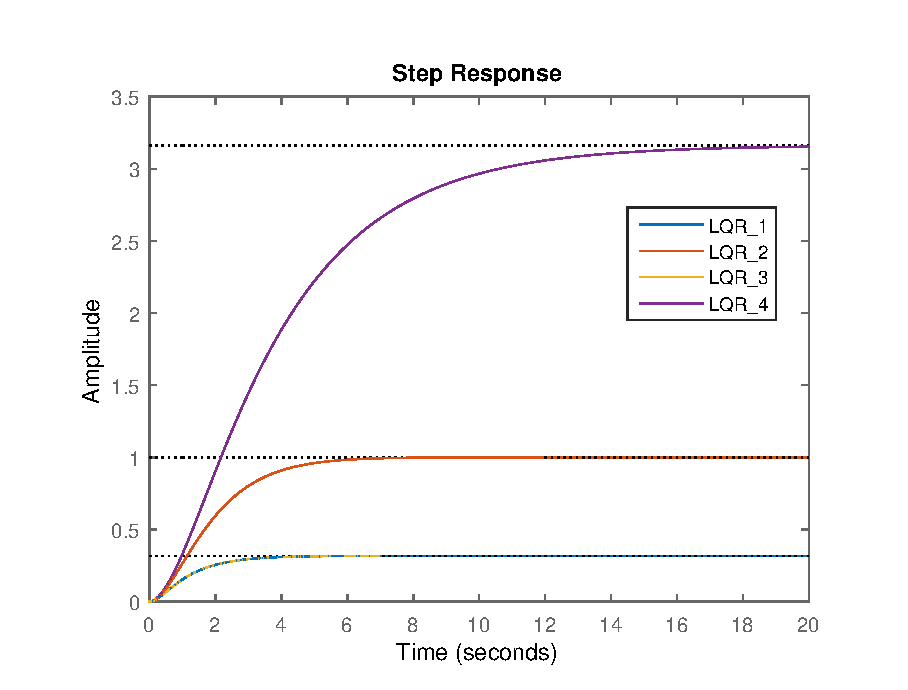
\includegraphics[width = 0.75\textwidth]{assets/image/PERBANDINGAN_PERFORMA.eps}
                    \caption{Perbandingan Performa Sistem dengan Variasi Nilai Q dan R}
                    \label{perbandingan_performa}
                \end{figure}
                Dari hasil pengujian \textit{step} diatas, dapat diamati bahwa data LQR 1 dan data LQR 3 saling berhimpit dan menunjukkan performa sistem paling baik karena memiliki rise time dan settling time yang cepat dibandingkan \textit{output} sistem lainnya.
   \section{Kesimpulan}
        Dari hasil dan pembahasan diatas didapat kesimpulan sebagai berikut,
        \begin{enumerate}
            \item Kendali LQR dapat digunakan untuk memanipulasi karakteristik sistem
            \item Penguatan pada sistem dapat menghilangkan \textit{error steady state}
        \end{enumerate}
    \begin{thebibliography}{1}
        \bibitem[1]{Fahmizal} Fahmizal. 2020. "Linear Quadratic Regulator (LQR)" dalam \textit{Modul Praktikum Teknik Kendali Lanjut} (hlm.1-4). Yogyakarta
    \end{thebibliography}
\end{document}